\chapter{Introduction}\label{chap:intro}
\setlength\epigraphwidth{.8\textwidth}
\epigraph{The night Max wore his wolf suit and made mischief of one kind\\
  and another\\
  his mother called him ``WILD THING!''\\
  and Max said ``I'LL EAT YOU UP!''\\
  so he was sent to bed without eating anything. }{---Maurice Sendak,
  \emph{Where the Wild Things Are}}

Before we begin: if the reader has not yet read the
\hyperlink{chap:preface}{preface}, we would like to take this
opportunity to mention its existence. Among other things, it contains
a \hyperlink{tab:notation}{table of notation} (\cref{tab:notation})
and a \hyperlink{pref:formatting}{brief note} on the formatting of the
document.

\section{Two Overviews of the Project}\label{sec:two-overviews}
We will give two birds-eye views of some of the questions we've
examined over the course of this project. The first
(\cref{subsec:chronological-overview}) is presented in
\emph{chronological} order, so as to capture more of the overarching
motivation to the topics we pursued. We hope this will help to ground
the reader in a sense of how each component of the project grew out of
the previous ones, and that it can also help orient new researchers
who are investigating similar questions to the ones we pursued. Note,
by virtue of this choice in presentation, it might be harder to get a
sense for ``where things are going'' while reading this section.

To address this, the second (\cref{subsec:more-explicit-description},
\cpageref{subsec:more-explicit-description}) contains more technical
detail, and stays much closer to the final layout of topics within the
document. Essentially, it is meant to function as an annotated table
of contents, listing big takeaways and/or theorems from each section
of the report. It is also much terser than the first, owing to its
different objective.

Naturally there is some redundancy between these two summaries, but we
hope that their different focuses will afford clarity to the reader in
navigating the content. On a final note, we should mention that
careful definitions of all the concepts presented below can be found
later; the ones here are occasionally given in loose terms to help
keep the pacing brisk.


\section{A Chronological Overview}\label{subsec:chronological-overview}

At the outset, our goals were as follows.
\begin{enumerate}[label=(\arabic*)]
  \item Give clear/engaging exposition on the foundations of knot
    theory, paying close attention to rigor.
  \item Explore the extent to which unknotting moves give us way to
    define new algebraic structure on the category of knots. In
    particular, we were interested in the loosely ``multiplicative''
    structure of the connected sum, and wanted to see if we could find
    an underlying ``addition'' operation corresponding to it.
\end{enumerate}
We leave it to the reader to judge our handiwork regarding (1).
Regarding (2), after a semester of largely-fruitless exploratory work,
it became clear that this was too ambitious for a 1-year
project.\footnote{That's not to say we did nothing --- we have some
  interesting exploratory results, but most of them are computational,
  as working theoretically turned out to hinge on the following
  example (which led us down the bottomless rabbit hole of \emph{wild
    knot theory}).}

However, there was at least one intriguing result that came out of our
attacks. In attempting to define all modifications of the Gauss code
in terms of group actions, we needed a way to treat all knots as if
they contained the same number of crossings. Essentially, this was
because we needed a way to interpret what ``flip crossing 17'' would
mean if we only had a 3-crossing knot. This led us to the following
example of a knot that \emph{appears} to be ambient-isotopic to the
unknot, despite having infinitely-many crossings (shown in
\cref{fig:pref-strange-unknot}).
\begin{figure}[H]
  \centering
  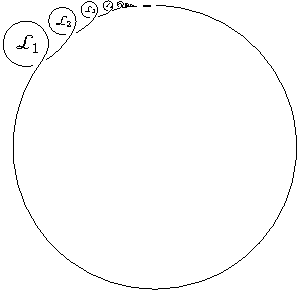
\includegraphics[width=.6\linewidth]{figures/rectifiable-knots/winf.pdf}
  \caption{A strange unknot\ldots}
  \label{fig:pref-strange-unknot}
\end{figure}
We'll show this is a valid embedding of $S^1$ when we talk about it in
depth in \cref{sec:countable-r1-moves-for-sn}.\footnote{In particular,
  see \cref{thm:countable-gluing-ambient-isotopies}} Note, the proof
we will give in that section differs from the sketch we're about to
describe; the latter came first chronologically (and ends up being a
bit more powerful), but is messier to work with.

Anyways: The loose idea is that we can create a uniformly convergent
sequence of ambient isotopies yielding \cref{fig:pref-strange-unknot}
in the limit. We can show that the associated homeomorphisms are
uniformly convergent, and that their inverses are as well. Then, after
arguing bijectivity, we can apply the fact that a uniform limit of
continuous functions is continuous to get a homeomorphism in the
limit. Finally, we apply a uniform convergence argument to the overall
ambient isotopy to show it is continuous.

% The loose idea is
% that we can realize \cref{fig:pref-strange-unknot} by looking at a
% countable sequence of ambient isotopies that act on disjoint sets of
% decaying diameter. Because the sets are all disjoint, we don't lose
% bijectivity in the limit, and because the diameters decay, we can
% argue continuity is preserved as well.\footnote{This is actually not
%   our original method of proof,


% }

%   In any case: later, we pursue a similar result, but drop the
%   assumption of \emph{disjointess} and instead apply uniform
%   convergence (see \cref{prop:uniform-convergence}, in particular
%   \cref{thm:uniformly-convergent-ambient-isotopy}). It will be
%   \hypertarget{important-note-on-method}{\textbf{very important}} to
%   be careful in this approach, as there are some very-similar
%   looking knots where this strategy doesn't work (see
%   \cref{ex:fox-artin-curve}). In particular, without the
%   disjointness condition, sometimes we can lose bijectivity in the
%   limit in ways that are not obvious.



This example was particularly puzzling, as it seemed to create
inconsistencies in the common definitions of \emph{tame knots}, a
handful of which are given below:
\begin{commondef}\label{def:cdef1}
  We say a knot $K : S^1 \into \RR^3$ is \emph{tame} iff it is ambient
  isotopic to a polygonal knot.
\end{commondef}
\begin{commondef}\label{def:cdef2}
  We say a knot $K : S^1 \into \RR^3$ is \emph{tame} iff for every
  point $x$ on $K$, there exists a neighborhood $U_x$ such that the
  pair $(U_x, K \cap U_x) \cong $ the standard $(\mrm{ball},
  \mrm{diameter})$ pair.
\end{commondef}
\begin{commondef}\label{def:cdef3}
  We say a knot $K : S^1 \into \RR^3$ is \emph{tame} iff it can be
  thickened to an embedding of a solid torus.
\end{commondef}
\begin{commondef}\label{def:cdef4}
  We say a knot $K : S^1 \into \RR^3$ is \emph{tame} iff it has
  finitely many crossings.
\end{commondef}
In particular: we were claiming that our $K$ satisfied
\cref{def:cdef1} (which would also imply satisfying \cref{def:cdef2}),
but it was in no way obvious that it satisfied \cref{def:cdef3}.
Further, \cref{def:cdef4} seemed to be outright violated. Hence the
project shifted focus to examining the foundations of Knot Theory in
an attempt to verify
\begin{enumerate}
  \item Whether or not any inconsistency was actually present, and
  \item If so, where? If not, why didn't we think so?
\end{enumerate}
For (a), the first plan of attack was to try and determine whether
there was a flaw in our theorems. One was not forthcoming to
us.\footnote{Of course, this does not mean an error does not exist
  (the reader is encouraged to get in touch if the find a problem),
  but we are fairly confident in our techniques, especially given that
  we provided multiple approaches (E.g.,
  \cref{thm:countable-gluing-ambient-isotopies},
  \cref{sec:c1-countable-r1}).}

Having failed to find an error in our proofs (but being convinced at
the time that a flaw must exist), we set about trying to disprove our
claim by finding another context where the same technique yielded a
contradiction. This led us to the following example of
\cite{FoxArtin}, here drawn as an arc\footnote{An \emph{arc} is an
  embedding of $[0,1] \into \RR^3$ (as opposed to a knot, which is an
  embedding of $S^1 \into \RR^3$).} made of countably-many line
segments (\cref{fig:fox-artin-ce})
\begin{figure}[H]
  \centering
  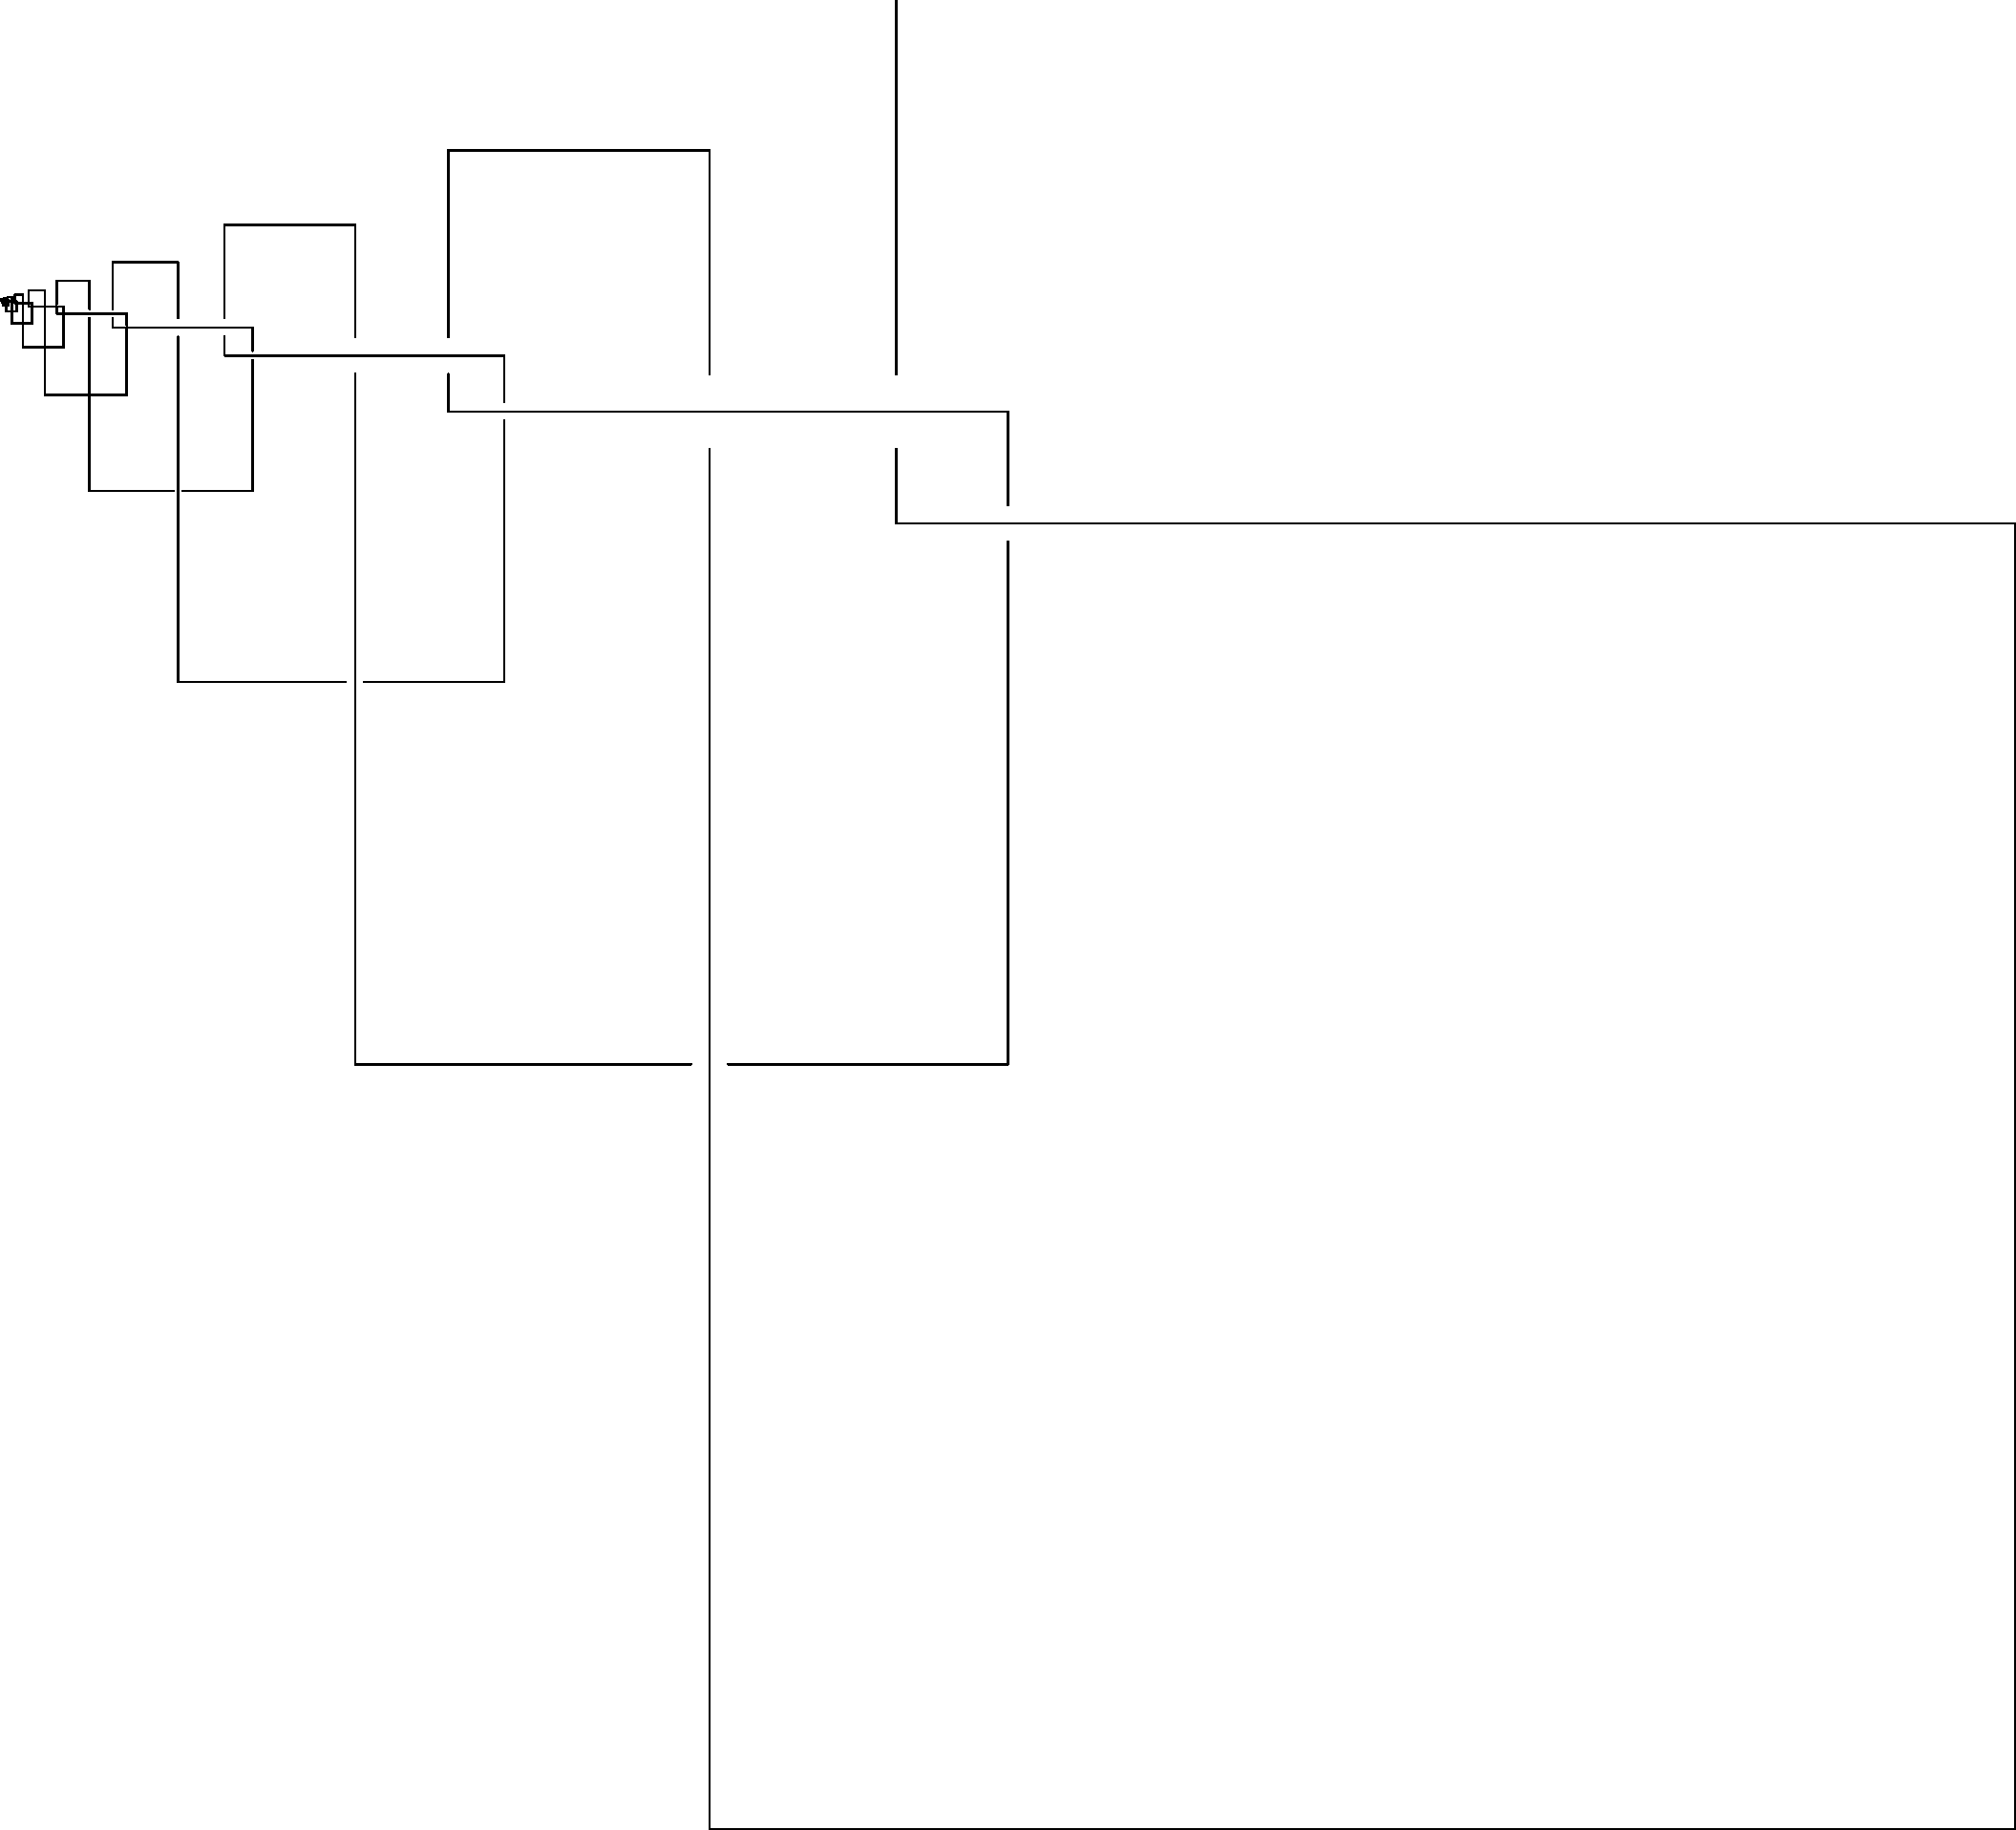
\includegraphics[scale=.19]{figures/preface/loops-no-boxes.pdf}
  \caption{The Wild Arc of Fox-Artin}
  \label{fig:fox-artin-ce}
\end{figure}
Interestingly, although it's possible to use Reidemeister II moves to
undo any finite number of the ``stitches'' in the above, this knot is
provably \emph{inequivalent} to any tame knot. To show this, Fox and
Artin developed an invariant for ``tameness'' based on the fundamental
group of a nested sequence of closed neighborhoods of the wild
point.\footnote{We reproduce their argument in
  \cref{ex:fox-artin-curve}.} The idea is that by showing that the
induced homomorphisms at each step are necessarily nontrivial, one can
show no ambient isotopy to a tame arc exists.

At this point, we took a deep dive into investigating the question of
when two \emph{arbitrary} knots are ambient-isotopic. In particular,
we wanted to know when we could use countable sequences of
Reidemeister moves. This became the focus of most the remainder of the
project.

As it turns out, this was far harder than we suspected. In fact,
across multiple books, papers, and conversations with knot theorists,
we heard sentiments like the following:
\begin{itemize}
  \item ``It would be fair to say that we know next to nothing about wild
    knots. Hence, we will not discuss them. We leave the problem to
    future generations.'' -An unnamed book
  \item ``I feel like I really know nothing about wild knots\ldots and
    I think most knot theorists would say the same (about themselves
    as well as me).'' -An unnamed knot theorist
  % \item ``If a wild knot embeds in $\RR^3$ and nobody cares, does it
  %   really exist?'' -Another mathematician
\end{itemize}
And so on. Further, a book we just recently discovered that treats the
general topic of embeddings of manifolds (\cite{Daverman}) has this to
say about the requirements for approaching the topic:
\begin{leftbar}
  ``What background is needed for reading this text? Chiefly, a
  knowledge of piecewise linear topology. [Although] to be honest, [we
  must also] presume extensive understanding of both general and
  algebraic topology [\ldots] as well. In an attempt to limit our
  presumptions, we [\ldots] shall take as granted the results from two
  fairly standard texts on general and algebraic topology [\ldots]
  each of which can be treated quite effectively in a year-long
  graduate course. Unfortunately, even [these] turn out to be
  insufficient for all our needs.''
\end{leftbar}
Naturally, all of this would be sure to strike fear into the heart of
any undergraduate attempting to tackle the problem, particularly one
who has yet to actually complete a single formal course in Topology.
Thus, it is a good thing we did not discover these problems until near
the completion of the project.

% {\color{blue} this isn't exactly true. I knew we didn't know a lot
% about wild knots, I just didn't
% know \emph{how much} we didn't know.}

% It gets worse. There \emph{is} a nice text that we just stumbled
% across while assembling our

% However, it turns out this does not actually provide us with a
% counterexample for our technique. After a lot of head-scratching, we
% discovered that there were some hidden problems in the Fox-Artin
% curve. The one we highlight here is that we lose bijectivity in the
% limit (we illustrate this in
% \cref{fig:fox-artin-pulling-out-a-stitch}), but it's worth noting that
% we also only get uniform convergence in the forward direction of our
% homeomorphism. Anyways, the point is that the problem was that the
% hypotheses of our theorems were not satisfied; the argument itself
% still seemed to hold.

Being blithely unaware of the dangers ahead, we forged dutifully
onward. Due to some confusion with the definition of a locally-finite
simplicial complex, we ended up focusing a large amount of our effort
on studying the question of which knots can be converted (through
ambient isotopy) to a countable union of polygonal segments. The
source of the confusion was as follows: If one ignores the weak
topology\footnote{Or, in our case, (a) simply does not know about its
  existence, followed in short time by (b) even upon learning about
  its existence, does not understand its significance} and views
simplicial complexes solely in terms of partitioning $\RR^n$, then it
becomes possible to find ``locally-finite'' ``simplicial complexes''
realizing many wild knots as chains of 1-simplices (with the wild
points being included as separate $0$-simplices). The prototypical
example is to do something like the following:
\begin{leftbar}
  For all $n \in \NN$, let $a_n = \set{\frac{1}{n+1}}$, $b_n =
  \set{\frac{1}{n}}$, and $I_n = \bk{\frac{1}{n+1}, \frac{1}{n}}$.
  Also let $I_\infty = \set{0}$. Then
  \[
    K = \set{I_\infty} \cup \bigcup_{n \in \NN} \set{a_n, b_n, I_n}
  \]
  satisfies the following properties:
  \begin{enumerate}
    \item For all $\sigma \in K$, every face $\tau$ of $\sigma$ is
      also an element of $K$
    \item For all $\sigma_0, \sigma_1 \in K$, if $\sigma_0 \cap
      \sigma_1 \neq \varnothing$, then $\tau = \sigma_0 \cap \sigma_1$
      is a sub-face of both $\sigma_0$ and $\sigma_1$, and
    \item For all $0$-simplices $\sigma \in K$, $\sigma$ is a vertex
      of at most finitely-many simplices in $K$.
  \end{enumerate}
\end{leftbar}
At first glance, one might protest that $I_\infty$ should really be a
face of \emph{infinitely-many} of the $1$-simplices. Morally, maybe
yes. But definitionally, no, this is actually not the case. $I_\infty$
is only incident in one simplex, namely itself. Indeed, one can see
that for all $n \in \NN$, $I_n \cap I_\infty = a_n \cap I_\infty = b_n
\cap I_\infty = \varnothing$. We can create analogues in higher
dimensions; E.g., an $\RR^2$ example is given by the following.
\begin{figure}[H]
  \centering
  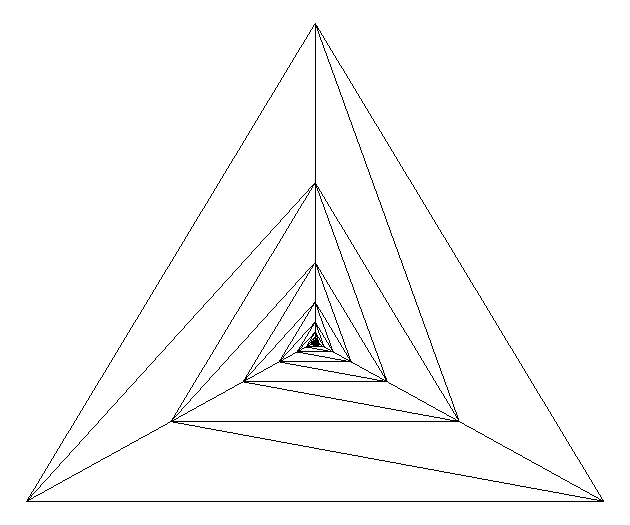
\includegraphics[scale=.5]{figures/wild/simp-comp-down.pdf}
  \caption{A ``locally-finite'' simplicial complex.}
\end{figure}
With this as motivation, we built up some formal machinery for working
directly with diagrams of wild knots provided that the crossing points
remain transverse and discrete.\footnote{For those familiar with the
  subject matter, this relaxes our axioms for ``regular diagrams'' to
  allow possibly \emph{countably} many crossings.} This allowed us to
show in \cref{thm:discrete-diagram-countably-polygonal} that
\emph{all} such knots are ambient isotopic to representatives
comprised of a countable union of polygonal segments. This was very
exciting, since it seemed it could open the door to attempting to
generalize Reidemeister's theorem to countable sequences of moves. We
already had an \emph{if} direction from
\cref{thm:uniformly-convergent-ambient-isotopy}; we were interested in
an \emph{only if}. Unfortunately, we did not have time to see it
through. This would be an interesting direction for future work.

Having taken a deep foray into the topic of wild embeddings \& built
up more machinery, at long last we returned back to our countable
Reidemeister I example, now much more confident in its correctness.
Using it as the cornerstone, we built up some basic definitions for
our desired algebraic framework (\cref{sec:defining-the-action}), and
created some basic tools for performing computational
search.\footnote{The code is available on Github:
  \url{https://github.com/redpanda1234/permutation-knots}}

We should emphasize that the primary strengths of this new formalism
do not stem from it delivering us a new understanding of the
equivalence problem (although its possible that connections will arise
in the future), but rather from the fact that it seems to offer a
natural language for studying unknotting moves. We would be very
interested in seeing future work in this direction.

This more-or-less wraps up the timeline for the project. In composing
this report, we were given an opportunity to reflect on what the
``heart'' of the project was. From the above, it might seem like an
answer is hard to glean, given the wide range of tangents we embarked
on. We would agree. In fact, we think that in it's own way, the
\np{``slipperiness'' of identifying the correct road forward in
  absence of established machinery} was the defining feature of our
work. We found that often, as soon as we stepped outside the scope of
Reidemeister's theorem, the standard intuition we used to approach
knot theory was fundamentally challenged at every turn. There were
many theorems we took for granted --- e.g., ``ambient isotopy and
ambient orientation-preserving homeomorphism are equivalent'' --- that
turned out to contain hidden PL hypotheses that we did not quite
understand the significance of. % Untangling this web of dependencies
% was the source of great confusion, but we.

Thus, in choosing how to present our findings, we decided to strive
for being as encyclopedic as possible, to help orient those interested
in future work. To that end we have placed particular attention on (a)
pointing out ways in which this perspective might be useful in
studying tame embeddings, (b) drawing attention to important
counterexamples that challenge our intuition, and (c) striving to be
maximally rigorous in working with our proofs.

% {\color{blue}
We hope they find the reader well.
% }

\section{The More Technical
  Overview}\label{subsec:more-explicit-description}
The document is structured as follows.
\begin{enumerate}[label=(\Roman*)]
  \item \cref{chap:intro}: In this chapter (which you are reading
    right now), we give two high-level overviews of the project,
    including one that has a more personal/chronological feel to it
    (\cref{subsec:chronological-overview}), as well as a more detailed
    ``table of contents,'' which includes, among other things, a
    recursive reference to its own contents
    (\cref{subsec:more-explicit-description}).
  \item \cref{part:fundamentals}: Fundamentals of Knot Theory. Here,
    we give an overview of the big picture ideas in knot theory, and
    list some basic definitions. We encourage those more familiar with
    the topics to read \cref{chap:motivation} but skip the rest.
    \begin{enumerate}[label=\arabic*)]
      \item In \cref{chap:motivation}, we discuss the knot equivalence
        problem, with particular focus on an analogy with determining
        equivalence of arithmetic expressions. We discuss the
        differences between these two contexts (e.g., the absence of a
        good simplification algorithm for knots), as well as what
        kinds of additional structure on the knot category might help
        get around some of these difficulties in the future. This
        serves to motivate the approach taken in
        \cref{chap:connections-to-sn}
      \item In \cref{chap:knots-and-knot-diagrams}, we provide the
        standard definitions for knots, ambient isotopy (highlighting the
        problems with choosing something like \emph{isotopy} instead
        as our definition of equivalence), tameness, regular diagrams,
        orientation, and so on. This is targeted mainly at those who
        are new to the topic; experts will probably find nothing
        surprising. One thing of note is that we place emphasis on
        highlighting the fact that going from ``working with knots''
        to ``working with knot diagrams'' should not be taken for
        granted.
    \end{enumerate}
  \item
    \cref{part:unknotting-moves-and-combinatorial-representations}:
    Combinatorial Representations. Here, we discuss what we call
    \emph{combinatorial representations}, i.e.\ ways of abstracting
    information in knot diagrams to strings that can be manipulated
    purely algebraically / combinatorially.%  The overarching desire is
    % to
    % to find a nice rule-based framework
    % Our prototypical (and in
    % fact, only) example is the signed Gauss code. We discuss
    \begin{enumerate}[label=\arabic*)]
        \setcounter{enumii}{3}
      \item In \cref{chap:gauss-code}, we introduce the signed Gauss
        code for a knot diagram. We discuss the Gauss code encoding of
        Reidemeister moves, especially the planarity constraint of
        Reidemeister II. A significant portion of the exposition is
        dedicated to discussing what we have called the \emph{diagram
        graph} (\cref{def:diagram-graph}), which is a graph
        constructed from the Gauss code that is particularly natural
        for computational manipulation. In particular, we prove that
        it has a unique planar embedding, and thus can be used to
        verify proposed Reidemeister II moves (we give a sketch for a
        greedy algorithm performing this check).

        Finally, we finish by introducing virtual knots as a way to
        avoid the planarity concerns of Reidemeister II, and work
        instead in a more purely combinatorial context. Discussion of
        the forbidden moves leads us to \emph{briefly} mentioning
        unknotting moves, and the intriguing sense in which they
        encode ``recipes'' for how to build knots from the unknot.
      \item In \cref{chap:connections-to-sn}, motivated by the
        discussion of unknotting moves, we build up basic definitions
        for our formalism that connects Gauss codes to actions of the
        symmetric group on a countable set. The desire here is to
        flesh out the idea of unknotting moves as ``building'' knots
        and ``converting them into each other.'' Unfortunately, it
        seems like on a purely theoretical level, it's not possible
        to reconcile knot equivalence with the group structure in a
        sensible way. Nonetheless, we did see some unexpected patterns
        in performing computer searches with \texttt{sage}.

        Underpinning all of our results in this chapter is the example
        of an unknot with a countable number of crossings. To show
        this is valid, we use a slightly simpler version of the
        uniform convergence proof we give later
        (\cref{thm:uniformly-convergent-ambient-isotopy}). To be extra
        sure that the result is valid (even if our proof turns out to
        secretly contain a flaw), we construct a $C^1$ embedding for
        our example of interest (\cref{sec:c1-countable-r1}),
        which suffices to guarantee it is tame (see
        \cref{chap:feral-gallery}).
        % In terms of a purely theoretical approach, it seems very
        % challenging to
        % Indeed, although we do not explicitly discuss this, one can
        % view unknotting moves as families of elements that
        % ``complete'' the Reidemeister moves in the sense of making
        % them sufficient to generate the entire group.
    \end{enumerate}
  \item In \cref{part:wild-knots}, we shift our focus to general
    topological embeddings, withe the goal of getting a better
    understanding our examples of countable Reidemeister I moves.
    \begin{enumerate}[label=\arabic*)]
        \setcounter{enumii}{5}
      \item In \cref{chap:tame-and-wild-knots}, we clarify common
        definitions for tameness and wildness that we have found in
        the literature, reconciling those that we can with the terms
        used when studying more general embeddings of $m$-manifolds
        into $n$-manifolds. We try to be particularly cognizant of
        which category we are working in at all times.
      \item In \cref{chap:machinery}, we begin building up machinery
        for our later work in studying ambient isotopy for general
        topological embeddings. We develop two tools (strand
        separation and uniform converence) which prove useful for
        working with wild knots whose wild points are topologically
        discrete. We do not build machinery for working with
        everywhere-wild knots.
      \item In \cref{chap:ambient-isotopy-in-r2}, we apply these tools
        in the case of $\RR^2$, and show that all curves $K : S^1
        \into \RR^2$ are ambient isotopic (this will be important when
        we move to $\RR^3$ in \cref{chap:moving-into-r3}). In
        \cref{sec:feral-points}, we discuss the pathologies that can
        arise in diagrams in $\RR^2$, which we refer as \emph{feral}
        behavior.
      \item In \cref{chap:moving-into-r3}, we use the techniques of
        \cref{chap:machinery} and \cref{chap:ambient-isotopy-in-r2} to
        study ambient isotopies in $\RR^3$. The loose idea is that as
        long as the crossing points in our diagrams are toplogically
        discrete, we have a bunch of strands that essentially act like
        they're curves embedded in $\RR^2$ (because, after all, they
        don't cross). This reduces the behavior to results covered by
        \cref{chap:ambient-isotopy-in-r2}. By then showing we can also
        constrain the behavior of our embeddings \emph{near} crossing
        points, we can then show that if a wild knot has a diagram
        with topologically discrete crossings, then it is ambient
        isotopic to a representative comprised of a countable union of
        polygonal segments. We conclude with some directions for
        future work, and offer a very brief sketch of how one might
        build an analogue to Reidemeister's theorem in this context.
      \item Lastly, in \cref{chap:summary}, we summarize the results
        of the project, and discuss possible ways of turning our
        ``crossing-discrete wild knots'' into a category more directly
        analogous to the PL case. This concludes the main body of the
        document.
    \end{enumerate}
  \item \cref{part:appendix} is the appendix. Here, we include some
    miscellany that didn't fit particularly well into any parts of the
    main document.
    \begin{enumerate}
      \item[A)] \cref{chap:feral-gallery} contains two extra feral
        knots that we have parameterized by a $C^1$ embedding.
      \item[B)] \cref{appendix:pl-topology} contains a basic
        crash-course in PL Topology, with an emphasis on the ``crash''
        part.
      \item[C)] \cref{chap:misc} includes misc.\ data from the
        project. This includes tables for the cycle representations
        computed in \cref{chap:connections-to-sn}.
    \end{enumerate}
\end{enumerate}


% The following gives





















% Anyways: As discussed in the preface, the original goals of the thesis
% were (1) to give lucid exposition on the fundamentals of knot theory,
% and (2) to study unknotting moves and how they might offer more
% explicit algebraic structure for knots.

% Regarding (1), we've sought to place particular emphasis on two
% points:
% \begin{enumerate}[label=\roman*)]
%   \item The material should be accessible to readers who don't
%     yet have extensive background in the field. Importantly,
%     ``accessible'' here does not mean eschewing rigor, but rather
%     taking care to motivate it properly.%  Instead, we
%     % have attempted to offer intuition for every definition given, as
%     % well as counterexamples illustrating why these particular
%     % definitions are ``the right ones.''
%   \item The exposition should try and communicate just as much
%     \emph{excitement} as it does technical content.
% % In addition to communicating understanding of the material,
% %     the exposition should give a sense for what makes the subject
% %     interesting. The hope is that the reader
% \end{enumerate}
% In short, the goal is to equip the reader with knowledge and convince
% them to explore further on their own. We chose to focus on a concept
% that we would personally have benefited from seeing emphasized early
% on in our investigation of knot theory; namely, the distinction
% between \emph{knots} and \emph{knot diagrams}. This topic is of
% central importance later on in the document, so we think focusing on
% it here is appropriate. In our descriptions, emphasis is placed on the
% use of pictures, as well as analogies with other mathematical
% concepts.

% Regarding (2): As we discovered, this goal was a bit too ambitious to
% take on during our limited timeframe. However, we still believe it
% represents a promising direction for future work, and hence have
% included some discussion of our motivation as well as some of our
% exploratory work.

% The main idea is to consider virtual knots as equivalence classes of
% elements of the finitary symmetric group on a countable
% set.\footnote{Of course, the equivalence relation is prohibitively
%   expensive to compute (since otherwise we'd have an efficient
%   solution to the knot equivalence problem).
%   % but the representation
%   % has the interesting property of giving us a new notion of ``knot
%   % multiplication.''
% } The correspondence is established in such a way that the Gauss code
% can be understood as an action of these permutations on a standard
% infinite sequence of string characters, by identifying the portions of
% the sequence that have been deranged from standard position. One
% interesting side-effect of this encoding is we can now define a new
% group-like operation on knots, namely composing the representing
% permutations. When we do so, we see that the action of these ``product
% knots'' on the standard sequence often yields Gauss codes that
% represent link diagrams.\footnote{In fact, simply looking at the
%   number of components in these link diagrams (not even their
%   connectivity) distinguished all but a handful of knots up to $8$
%   crossings. However, this could be a superficial result since we made
%   no attempts to examine ways of normalizing the effects of
%   Reidemeister moves, so this is not even an invariant.} We would be
% curious to see whether this provides a new interpretation for bracket
% polynomials, such as those in our previous work
% (\cite{Kobayashi2019Sep}).
% % 'll see that there are some connections between
% % \np{algebraic properties of knots} and \np{permutation groups}.
% % {\color{pink} This will come in the form of some sort of isomorphism.}
% % Tame knots can be thought of in terms of the \emph{finitary symmetric
% %   group} (all finite permutations on $\NN$), while wild knots whose
% % \np{sets of wild points are topologically discrete} can be understood
% % as arbitrary elements of $\ms S_{\NN}$. We have not investigated
% % similar ideas for knots that are everywhere-wild.}

% In establishing the connection described above, we'll see that it's
% important to come up with a diagramming system that gives every tame
% knot the same ``number'' of crossings. This is where the example of
% the unknot with countable Reidemeister I moves (see
% \cref{fig:pref-strange-unknot}, \cpageref{fig:pref-strange-unknot})
% comes into play. This (and similar examples) will comprise the
% remainder of the document, which represents a third goal on the list:
% \begin{enumerate}
%   \item[(3)] Gain a better understanding of wild knots.
% \end{enumerate}
% In this direction, first we will provide explanations of how our
% example can be reconciled with some of our intuitive definitions of
% what it means for a knot to be ``tame.'' In particular, we will
% construct an ambient isotopy to a \emph{PL knot}, show that there
% exists a \emph{smooth} knots realizing diagrams like
% \cref{fig:pref-strange-unknot}, and give a sketch for how we can
% construct a lift from this countable Reidemeister I knot to an
% embedding of the solid torus $S^1 \times \mathbb{D}^2$.

% This led us to some further investigations of wild knots. To finish up
% the project, we prove a coarse sort of hierarchical result regarding
% the ``wildness'' of knots (again, using the invariant of
% \cite{FoxArtin}), and also develop a sketch of how to generalize
% Reidemeister's Theorem using arguments based on uniform continuity and
% / or uniform convergence.

% These three goals are each contained in a separate Part of the
% document. \cref{part:fundamentals} contains our exposition on the
% fundamentals of knot theory, \cref{part:unknotting-moves} contains our
% exploration of unknotting moves and combinatorial structures, and
% \cref{part:wild-knots} discusses the countable Reidemeister I moves in
% more detail, and also examines some aspects of the ambient isotopy
% problem for wild knots.

%%% Local Variables:
%%% TeX-master: "../../kobayashi-thesis"
%%% End:
